\section{Organisatorisches}

Prof. Flach, Raum Z436\\
flach@htw-dresden.de

\section{Einführung}

Herleiten von Gleichungen \Ra Zusammenhänge ersichtlich

\subsection{Ablauf}

Vorlesung 2x / Woche
\begin{itemize}
	\item Übung 1x / Woche
	\item Praktikum
	\item Prüfung 2-teilig
	\begin{itemize}
		\item Dezember 90 min
		\item Februar 90 min
		\item Nur Taschenrechner als Hilfmittel zugelassen
	\end{itemize}
	\item (Lernraum ET)
\end{itemize}

\subsection{Bedeutung der Elektrotechnik}

%TODO: Grafik digitalisieren
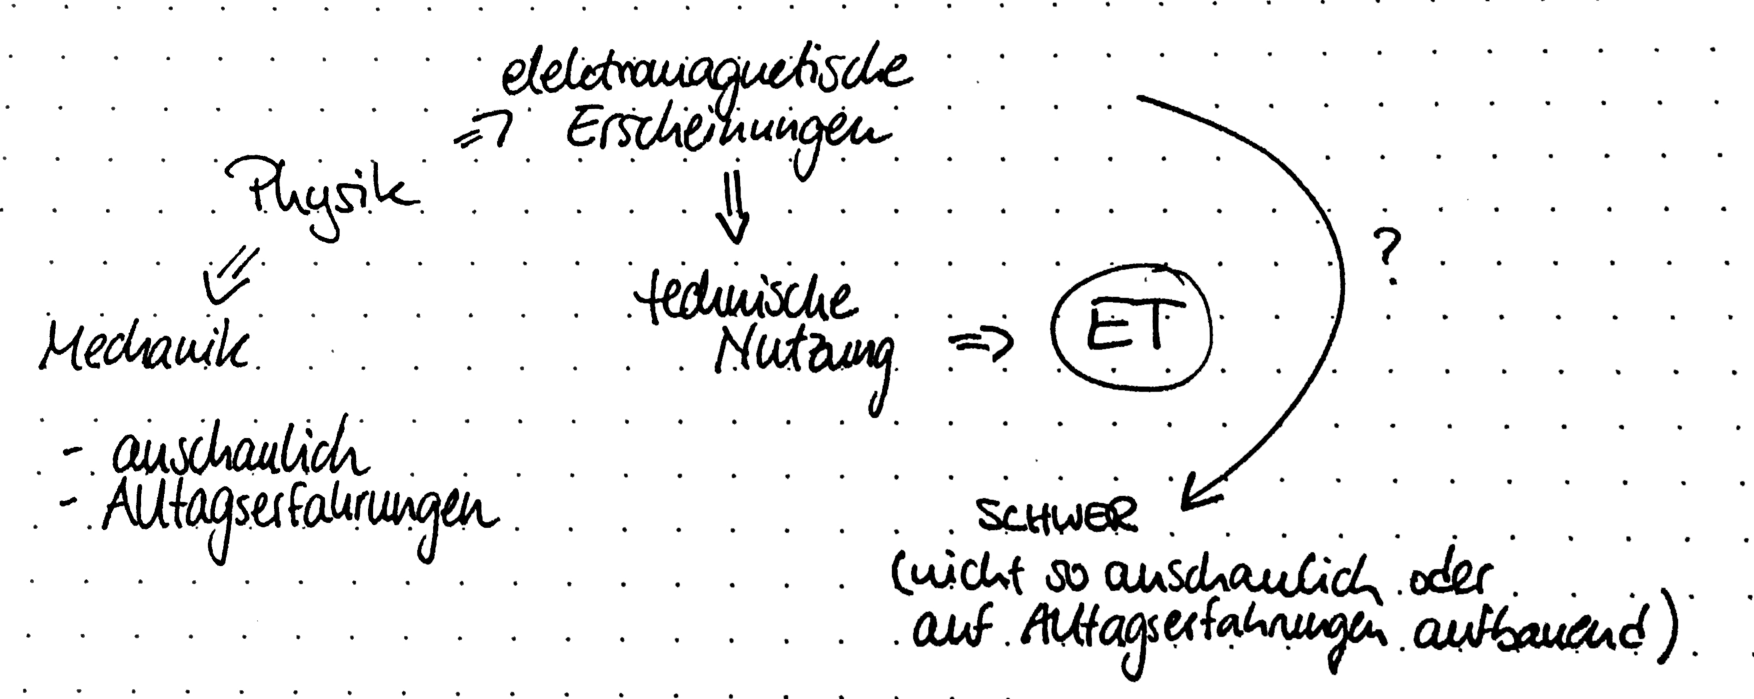
\includegraphics[width=\textwidth]{img/1_1}

\subsection{Fachsprache der ET}

Vereinbarung über Bestandteile + Regeln des Zusammenwirkens

\underbar{Beispiel:} Ohm'sches Gesetz:

\begin{itemize}
	\item verbal (physikalischer Zusammenhang)
	\item Gleichung mit Formelzeichen\\
		$$R = \frac{U}{I}$$
\end{itemize}

U ist die unabhängige Variable \ra x-Achse.

\glqq Weil Spannung anliegt, fließt Strom.\grqq

%TODO: Grafik digitalisieren
\begin{center}
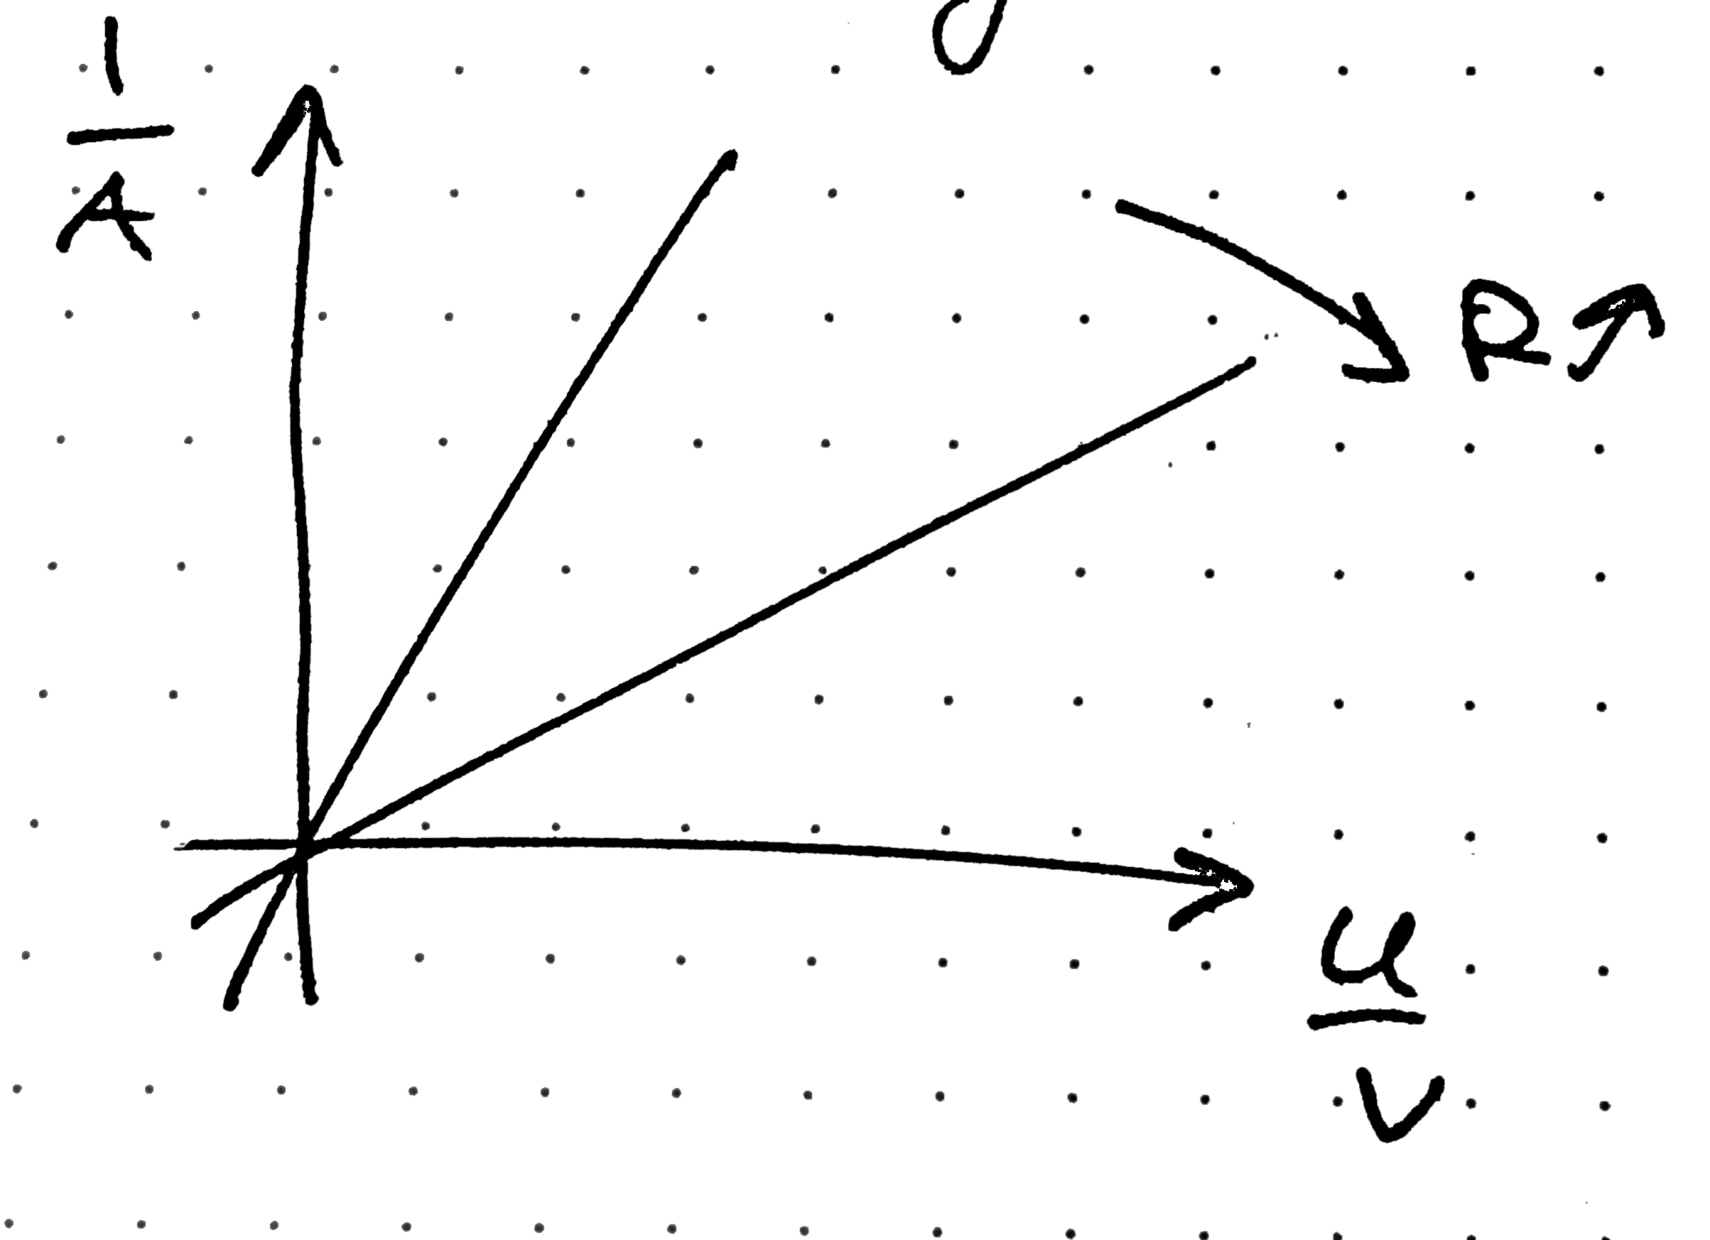
\includegraphics[width=0.5\textwidth]{img/1_2}
\end{center}

\underbar{Bestandteile:}
\begin{itemize}
	\item Formelzeichen für physikalische Größen 
		(Maßzahl, Vorsatzzeichen, Maßeinheit)\\
		I in A, U in V, R in m$\Omega$
	\item Gleichungen, bezogene Größengleichung
	\item graphische Hilfsmittel
\end{itemize}

\subsection{Einheiten in der Elektrotechnik}

SI-Einheiten (Masse, Länge, Zeit, Lichtstärke, Temperatur, Stoffmenge, elektrische Stromstärke)

%TODO: Grafik digitalisieren
\begin{center}
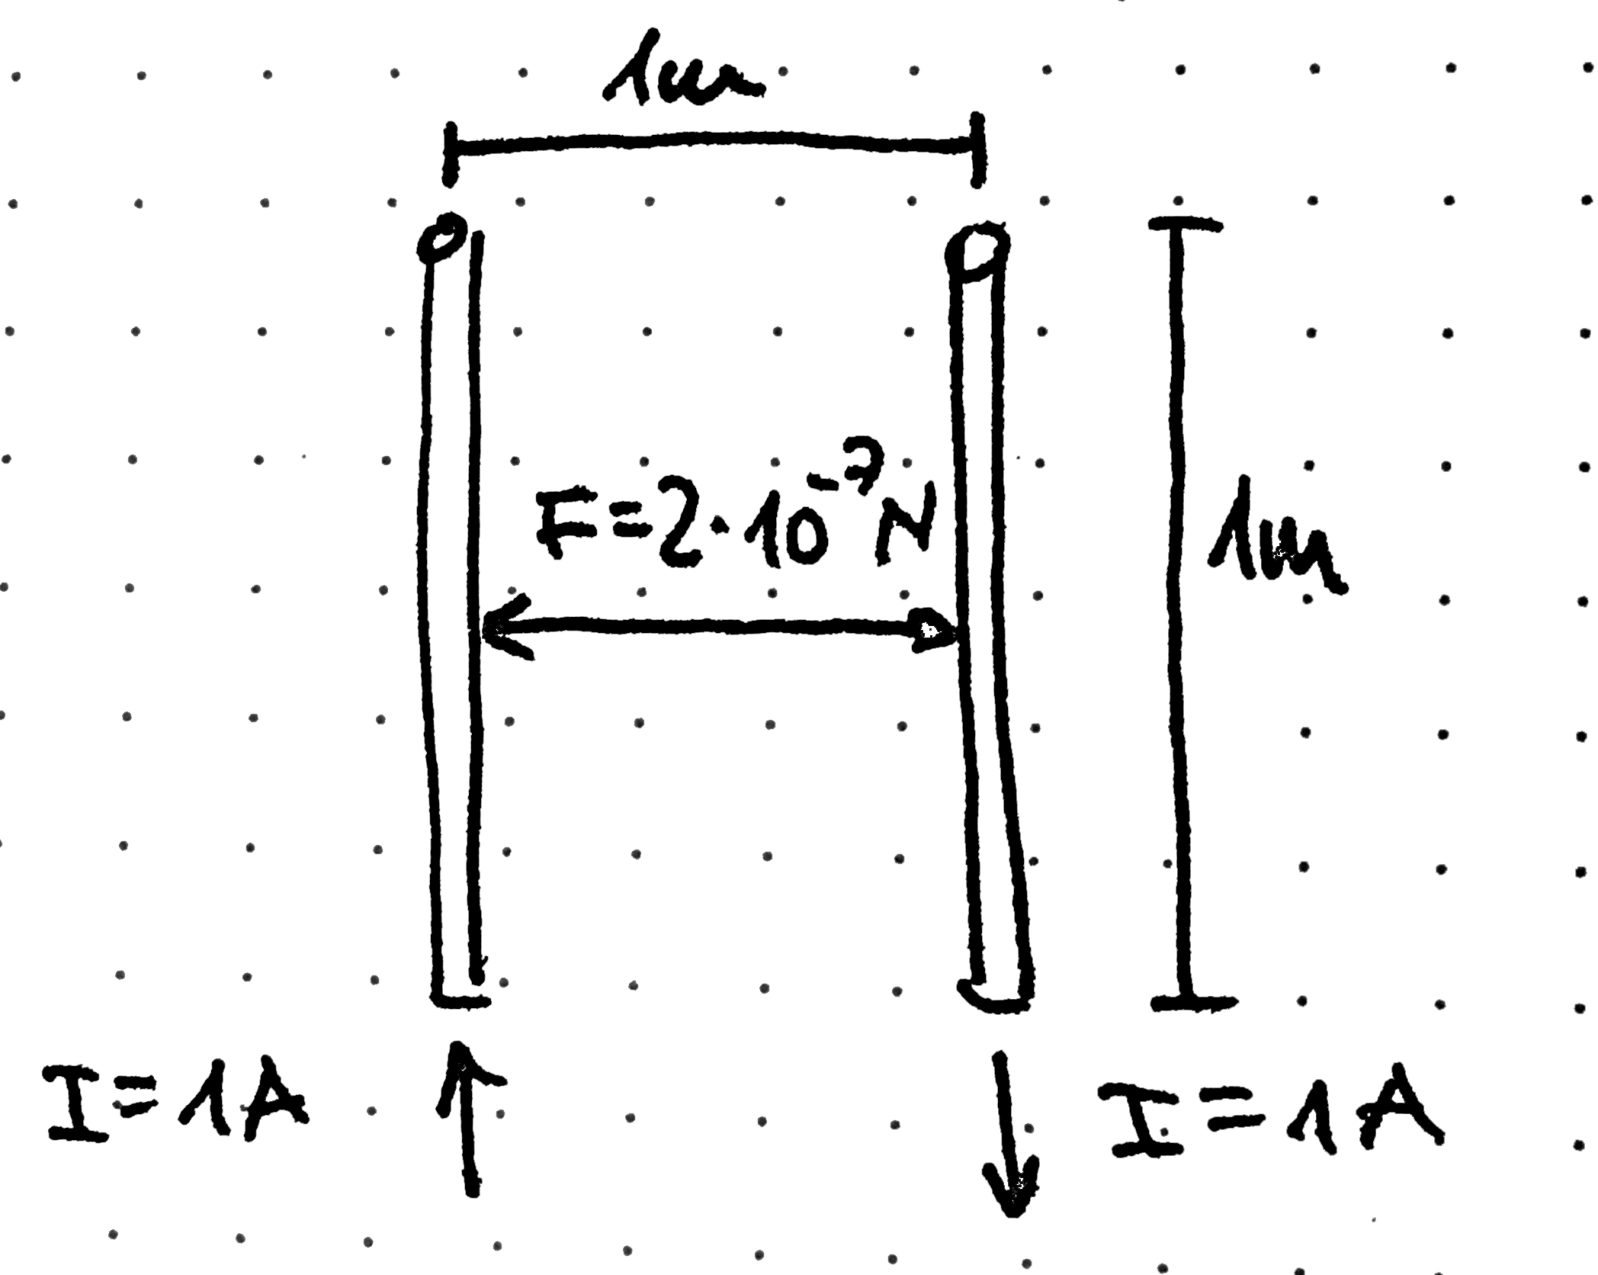
\includegraphics[width=0.5\textwidth]{img/1_3}
\end{center}
Definition von 1A

\section{Grundbegriffe der Elektrotechnik}
\subsection{Elektrische Ladung}

Strom $\hat{=}$ \glqq Elektrizitätsteilchen\grqq

\Ra Modell: 2 Arten von Ladungen\\
\ra positive + negative Ladungen \ra Elementarladung $e = 1,6 \times 10^{-19}C$ (oder $As$)

\Ra Bohr-Sommerfeld'sches Atommodell

%TODO: Grafik digitalisieren
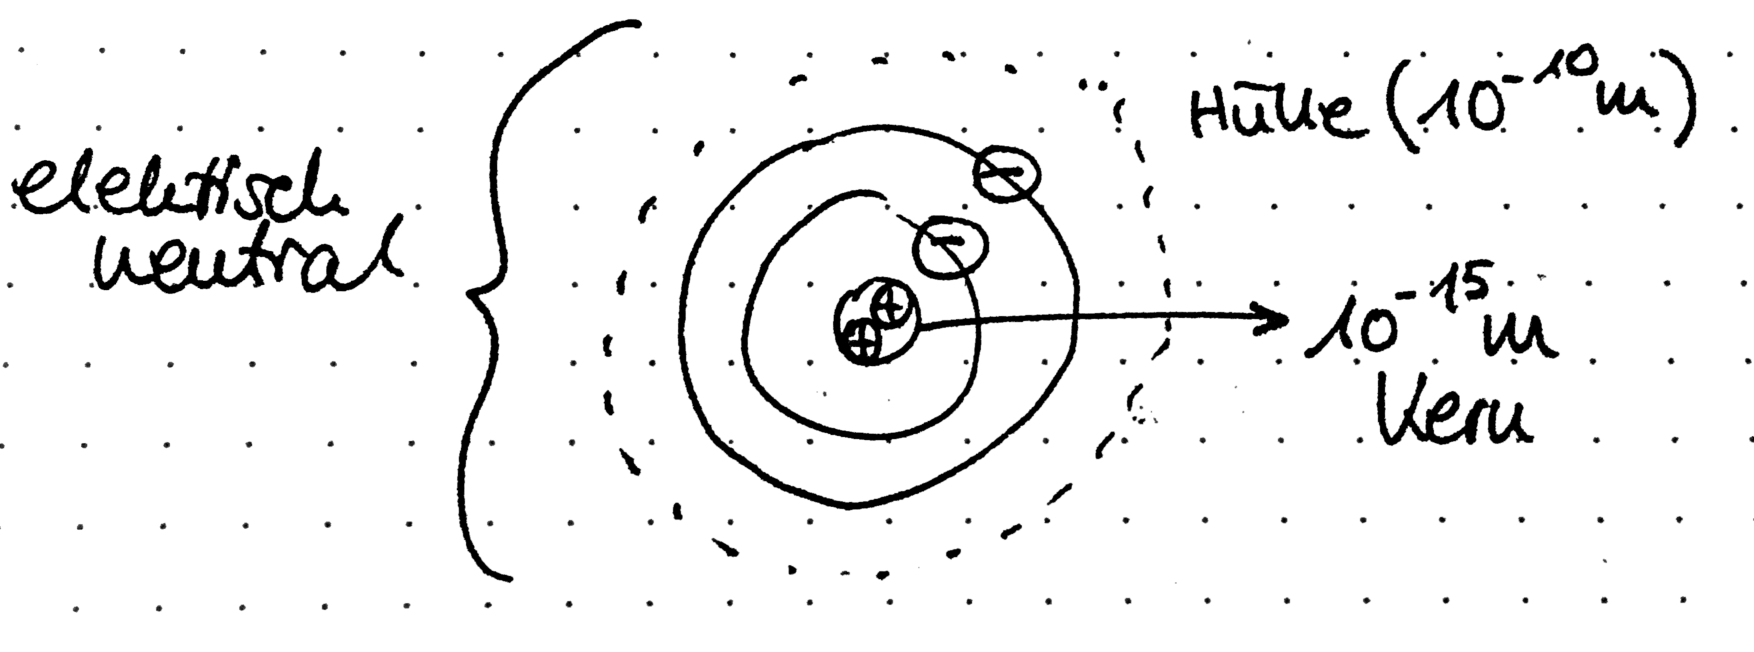
\includegraphics[width=\textwidth]{img/1_4}

Kraftwirkung zwischen Ladungen

Ladung versetzt den umgebenen Raum in einen bestimmten Zustand, den nennt man Feld (hier: elektrisches Feld).

Feld ist nicht an Materie gebunden.

Nachweis über Kraftwirkung

$$E = \frac{F}{Q}$$

elektrische Feldstärke = Kraft, die auf Ladung Q wirkt

keine Wirkung auf Masse, nur auf andere Ladungen.

\subsection{Leitungseigenschaften}

Nach Fähigkeit, elektrischen Strom zu leiten, werden Materialien in Leiter und Nichtleiter eingeteilt.

%TODO: Grafik digitalisieren
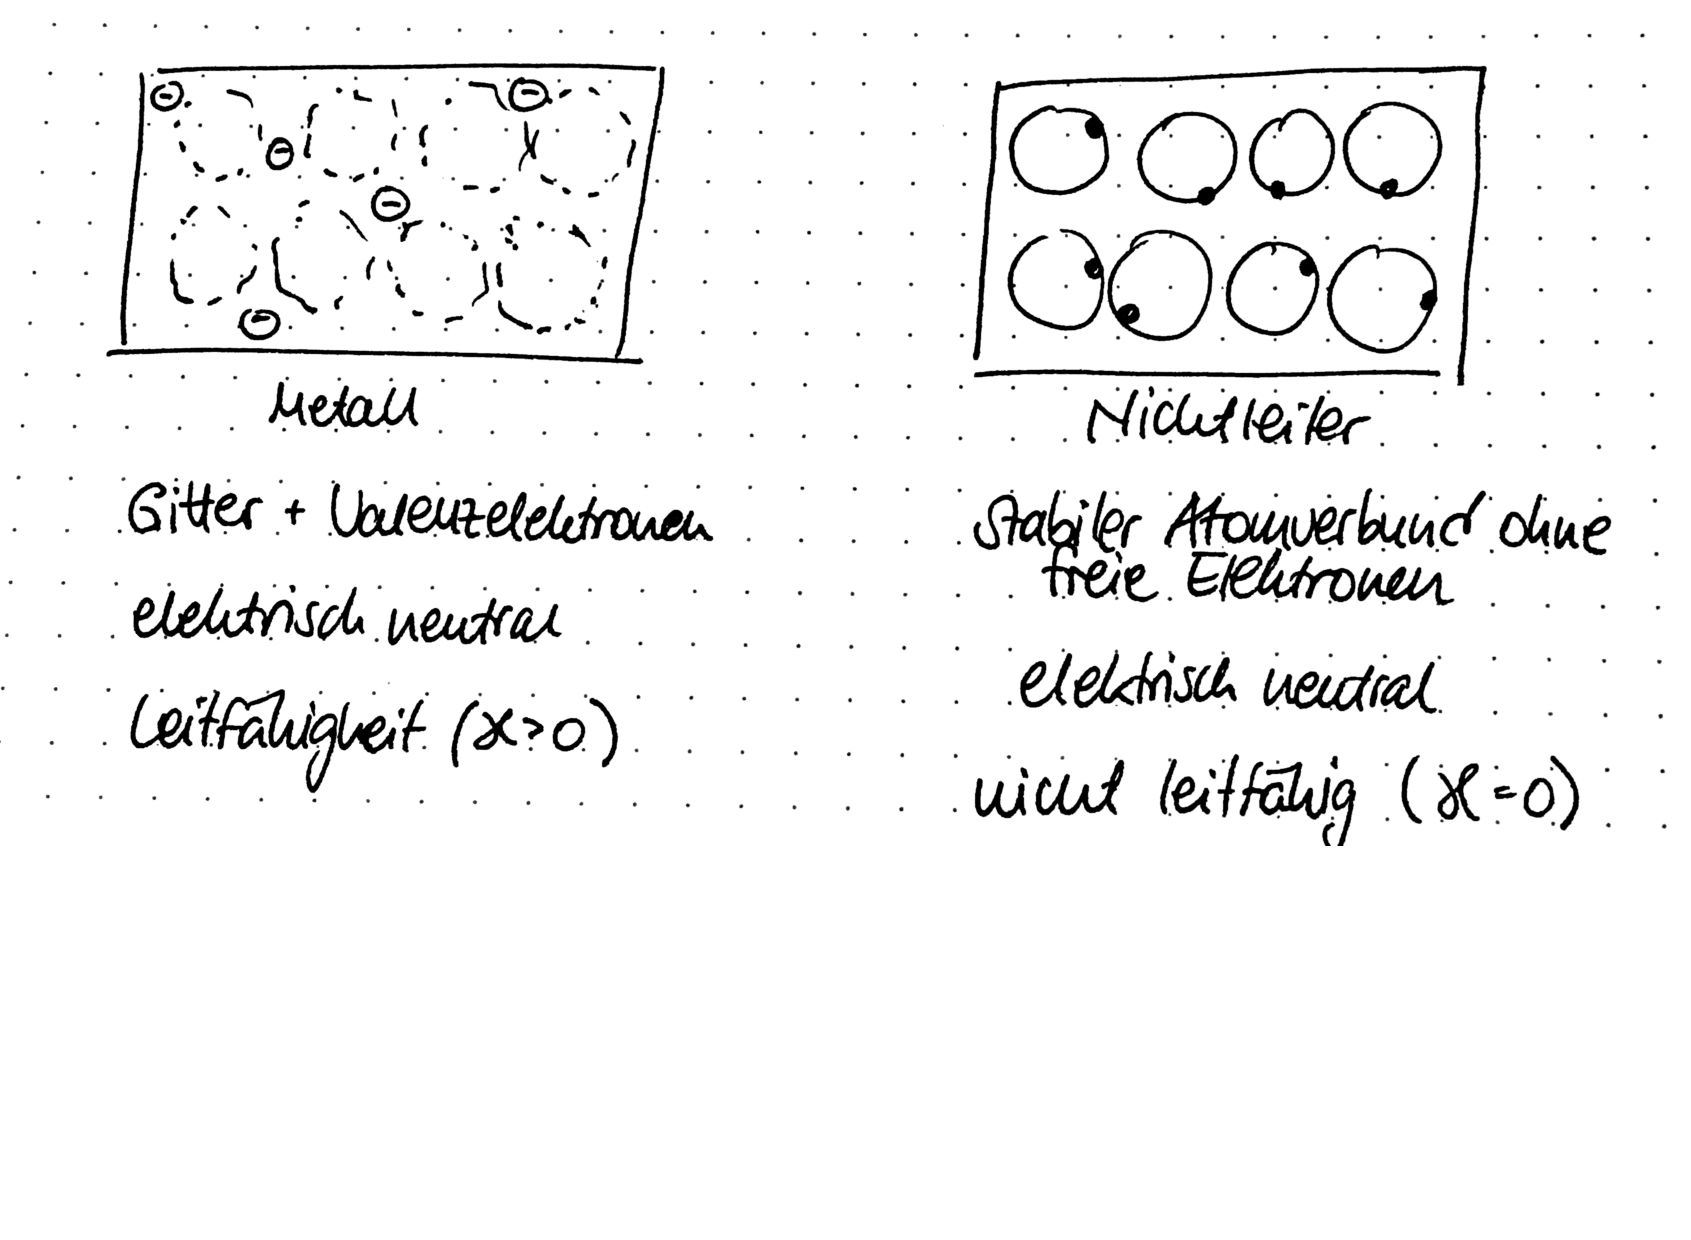
\includegraphics[width=\textwidth]{img/1_5}

Anzahl freier Ladungsträger für Cu: $n_n = 8 \times 10^{22}cm^3$

Metalle (Au, Cu, Ag, Al), Salzlösungen

\subsection{Elektrischer Strom, Stromdichte}

elektrischer Strom: Bewegung von Ladungsträgern (positiv \& negativ)

\underbar{Eigenschaften:}
\begin{itemize}
	\item positiver Strom (I > 0): Strom in Richtung der positiven Ladungsträger
	\item Stromstärke: Anzahl der Ladungsträger durch vorgegebenen Querschnitt pro Zeit\\
		$I = \frac{\Delta Q}{\Delta t} = \frac{Q}{t}$ \Ra Gleichstrom (falls konstant)\\
		$i(t) = \frac{\mathrm{d}Q}{\mathrm{d}t}$ \Ra zeitabhängiger Strom (sehr kleine Änderungen)
	\item Kontinuitätsgesetz:\\
		%TODO: Grafik digitalisieren
		\begin{center}
			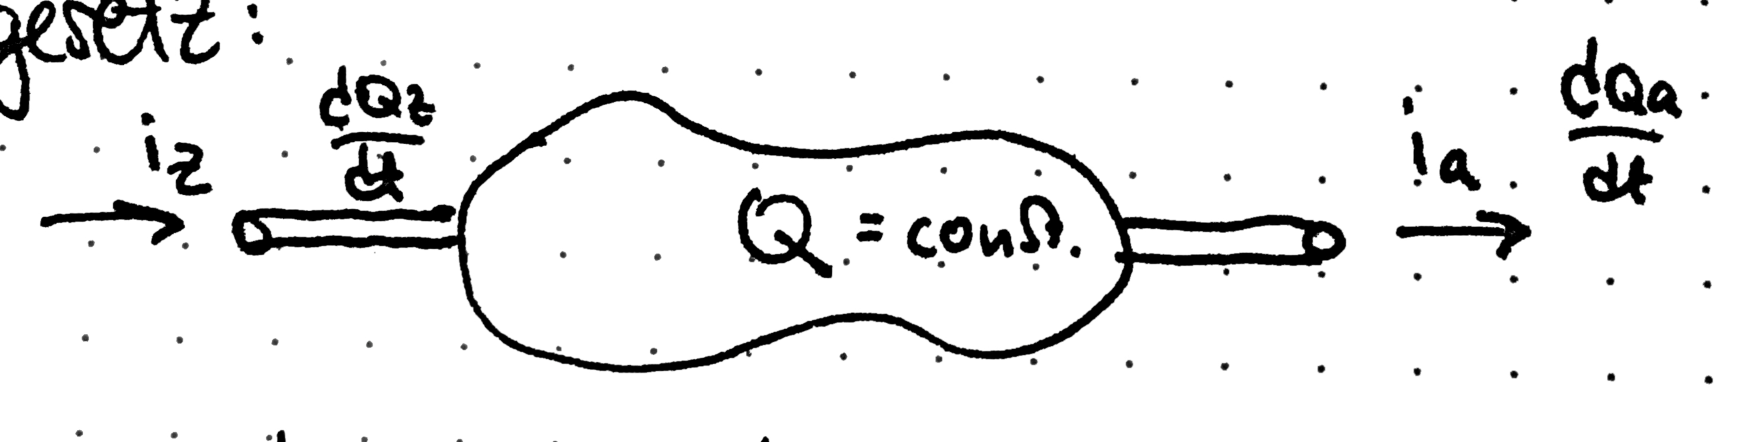
\includegraphics[width=0.7\textwidth]{img/1_6}
		\end{center}
		$$\frac{\mathrm{d}Q}{\mathrm{d}t}=0$$
		$$\frac{\delt Q_z}{\delt t} - \frac{\delt Q_a}{\delt t} = 0$$
		$$\Rightarrow i_z - i_a = 0$$
	\item Strom ist stets in sich geschlossen
	\item Wirkungen: Wärme, Magnetismus, chemische Wirkungen
\end{itemize}